\section{oosalizer/webalizer.c-Dateireferenz}
\label{webalizer_8c}\index{oosalizer/webalizer.c@{oosalizer/webalizer.c}}
{\tt \#include $<$time.h$>$}\par
{\tt \#include $<$stdio.h$>$}\par
{\tt \#include $<$stdlib.h$>$}\par
{\tt \#include $<$string.h$>$}\par
{\tt \#include $<$unistd.h$>$}\par
{\tt \#include $<$ctype.h$>$}\par
{\tt \#include $<$sys/utsname.h$>$}\par
{\tt \#include $<$sys/times.h$>$}\par
{\tt \#include $<$zlib.h$>$}\par
{\tt \#include $<$sys/types.h$>$}\par
{\tt \#include \char`\"{}webalizer.h\char`\"{}}\par
{\tt \#include \char`\"{}output.h\char`\"{}}\par
{\tt \#include \char`\"{}parser.h\char`\"{}}\par
{\tt \#include \char`\"{}preserve.h\char`\"{}}\par
{\tt \#include \char`\"{}hashtab.h\char`\"{}}\par
{\tt \#include \char`\"{}linklist.h\char`\"{}}\par
{\tt \#include \char`\"{}webalizer\_\-lang.h\char`\"{}}\par


Include-Abh\"{a}ngigkeitsdiagramm f\"{u}r webalizer.c:\begin{figure}[H]
\begin{center}
\leavevmode
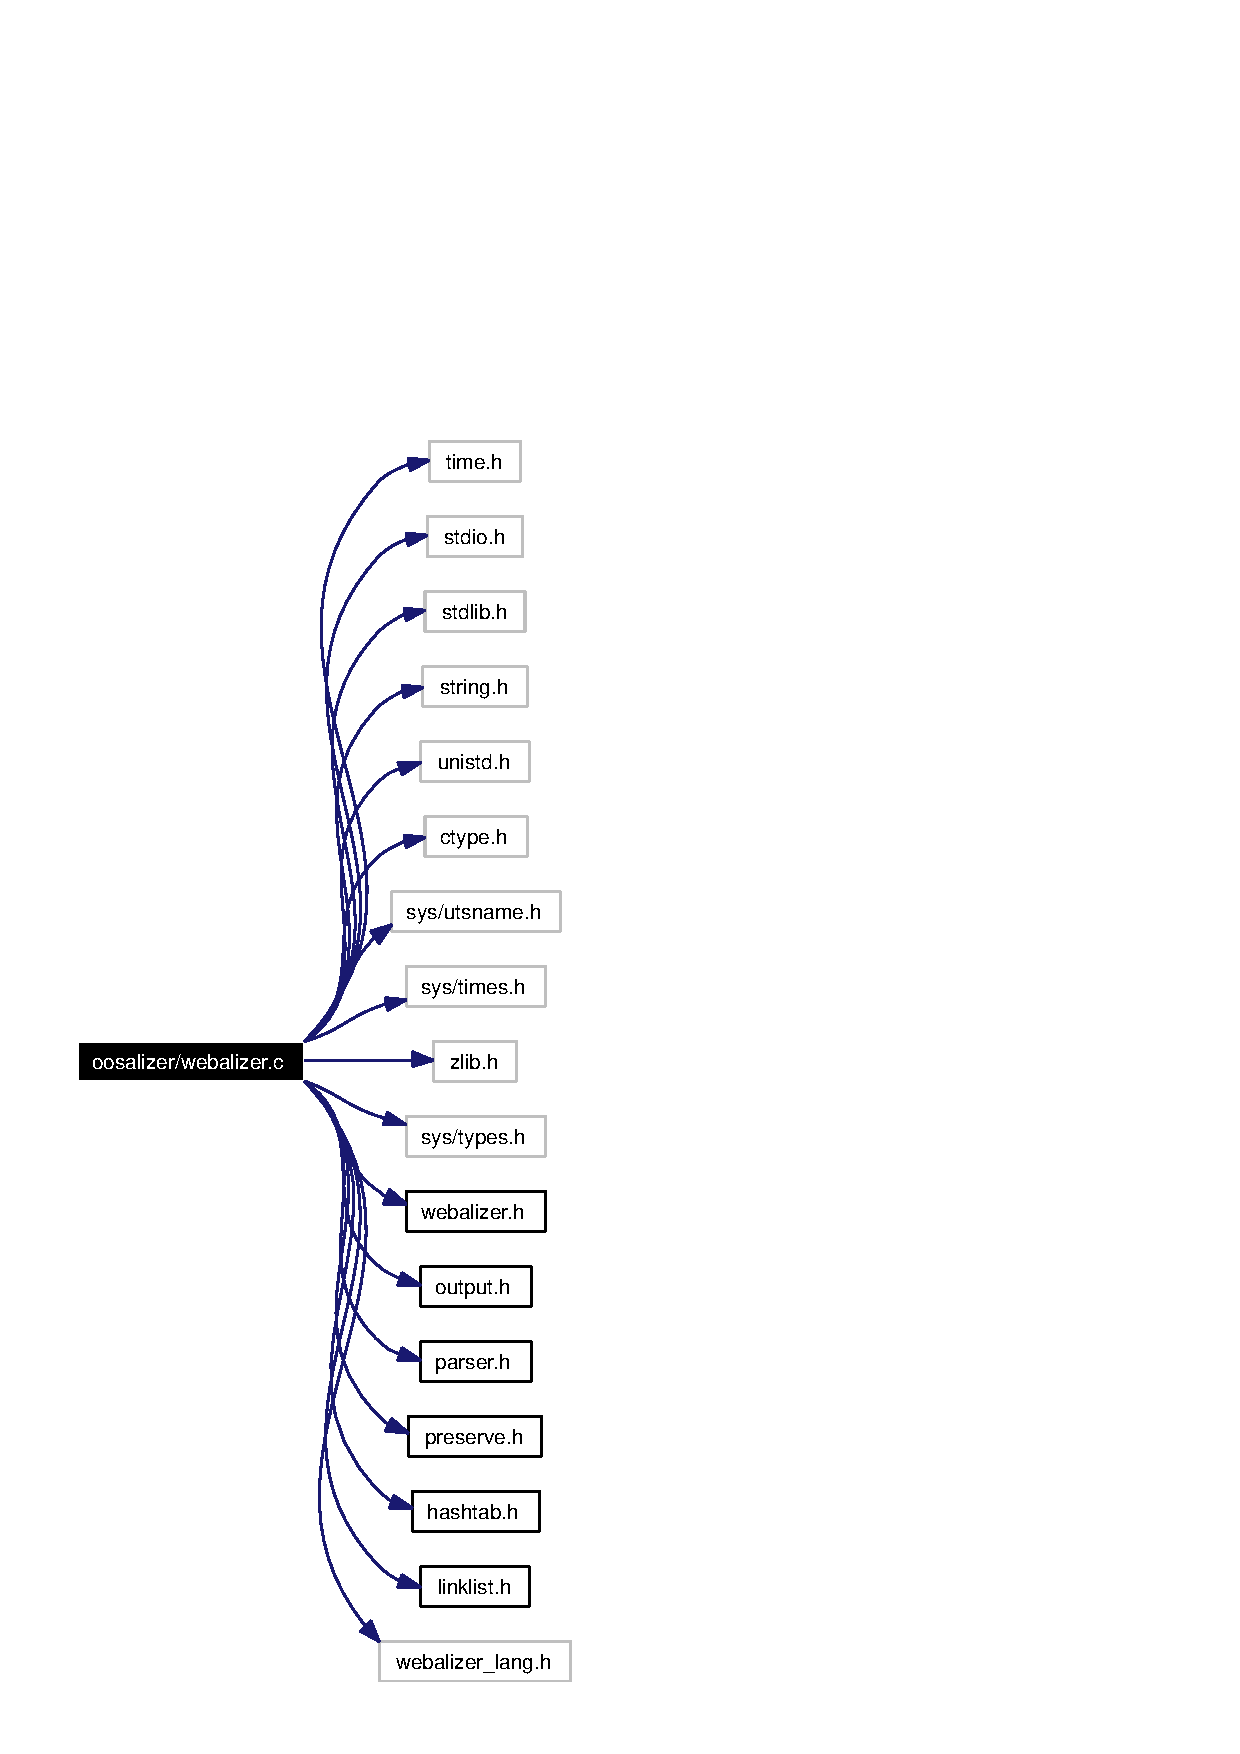
\includegraphics[width=137pt]{webalizer_8c__incl}
\end{center}
\end{figure}
\subsection*{Makrodefinitionen}
\begin{CompactItemize}
\item 
\#define {\bf CLK\_\-TCK}~\_\-SC\_\-CLK\_\-TCK
\item 
\#define {\bf GZ\_\-BUFSIZE}~16384
\end{CompactItemize}
\subsection*{Funktionen}
\begin{CompactItemize}
\item 
void {\bf clear\_\-month} ()
\item 
char $\ast$ {\bf unescape} (char $\ast$)
\item 
char {\bf from\_\-hex} (char)
\item 
void {\bf print\_\-opts} (char $\ast$)
\item 
void {\bf print\_\-version} ()
\item 
int {\bf isurlchar} (unsigned char)
\item 
void {\bf get\_\-config} (char $\ast$)
\item 
static char $\ast$ {\bf save\_\-opt} (char $\ast$)
\item 
void {\bf srch\_\-string} (char $\ast$)
\item 
char $\ast$ {\bf get\_\-domain} (char $\ast$)
\item 
char $\ast$ {\bf our\_\-gzgets} (gz\-File, char $\ast$, int)
\item 
int {\bf main} (int argc, char $\ast$argv[$\,$])
\item 
void {\bf init\_\-counters} ()
\item 
char $\ast$ {\bf cur\_\-time} ()
\item 
int {\bf ispage} (char $\ast$str)
\item 
u\_\-long {\bf ctry\_\-idx} (char $\ast$str)
\item 
u\_\-long {\bf jdate} (int day, int month, int year)
\end{CompactItemize}
\subsection*{Variablen}
\begin{CompactItemize}
\item 
char $\ast$ {\bf version} = \char`\"{}2.01\char`\"{}
\item 
char $\ast$ {\bf editlvl} = \char`\"{}10\char`\"{}
\item 
char $\ast$ {\bf moddate} = \char`\"{}16-Apr-2002\char`\"{}
\item 
char $\ast$ {\bf copyright} = \char`\"{}Copyright 1997-2001 by Bradford L. Barrett\char`\"{}
\item 
int {\bf verbose} = 2
\item 
int {\bf debug\_\-mode} = 0
\item 
int {\bf time\_\-me} = 0
\item 
int {\bf local\_\-time} = 1
\item 
int {\bf ignore\_\-hist} = 0
\item 
int {\bf hourly\_\-graph} = 1
\item 
int {\bf hourly\_\-stats} = 1
\item 
int {\bf daily\_\-graph} = 1
\item 
int {\bf daily\_\-stats} = 1
\item 
int {\bf ctry\_\-graph} = 1
\item 
int {\bf shade\_\-groups} = 1
\item 
int {\bf hlite\_\-groups} = 1
\item 
int {\bf mangle\_\-agent} = 0
\item 
int {\bf incremental} = 0
\item 
int {\bf use\_\-https} = 0
\item 
int {\bf visit\_\-timeout} = 1800
\item 
int {\bf graph\_\-legend} = 1
\item 
int {\bf graph\_\-lines} = 2
\item 
int {\bf fold\_\-seq\_\-err} = 0
\item 
int {\bf log\_\-type} = LOG\_\-CLF
\item 
int {\bf group\_\-domains} = 0
\item 
int {\bf hide\_\-sites} = 0
\item 
char $\ast$ {\bf hname} = NULL
\item 
char $\ast$ {\bf state\_\-fname} = \char`\"{}webalizer.current\char`\"{}
\item 
char $\ast$ {\bf hist\_\-fname} = \char`\"{}webalizer.hist\char`\"{}
\item 
char $\ast$ {\bf html\_\-ext} = \char`\"{}html\char`\"{}
\item 
char $\ast$ {\bf dump\_\-ext} = \char`\"{}tab\char`\"{}
\item 
char $\ast$ {\bf conf\_\-fname} = NULL
\item 
char $\ast$ {\bf log\_\-fname} = NULL
\item 
char $\ast$ {\bf out\_\-dir} = NULL
\item 
char $\ast$ {\bf blank\_\-str} = \char`\"{}\char`\"{}
\item 
char $\ast$ {\bf dns\_\-cache} = NULL
\item 
int {\bf dns\_\-children} = 0
\item 
int {\bf ntop\_\-sites} = 30
\item 
int {\bf ntop\_\-sites\-K} = 10
\item 
int {\bf ntop\_\-urls} = 30
\item 
int {\bf ntop\_\-urls\-K} = 10
\item 
int {\bf ntop\_\-entry} = 10
\item 
int {\bf ntop\_\-exit} = 10
\item 
int {\bf ntop\_\-refs} = 30
\item 
int {\bf ntop\_\-agents} = 15
\item 
int {\bf ntop\_\-ctrys} = 30
\item 
int {\bf ntop\_\-search} = 20
\item 
int {\bf ntop\_\-users} = 20
\item 
int {\bf ntop\_\-notfound} = 50
\item 
int {\bf all\_\-sites} = 0
\item 
int {\bf all\_\-urls} = 0
\item 
int {\bf all\_\-refs} = 0
\item 
int {\bf all\_\-agents} = 0
\item 
int {\bf all\_\-search} = 0
\item 
int {\bf all\_\-users} = 0
\item 
int {\bf dump\_\-sites} = 0
\item 
int {\bf dump\_\-urls} = 0
\item 
int {\bf dump\_\-refs} = 0
\item 
int {\bf dump\_\-agents} = 0
\item 
int {\bf dump\_\-users} = 0
\item 
int {\bf dump\_\-search} = 0
\item 
int {\bf dump\_\-header} = 0
\item 
char $\ast$ {\bf dump\_\-path} = NULL
\item 
int {\bf cur\_\-year} = 0
\item 
int {\bf cur\_\-month} = 0
\item 
int {\bf cur\_\-day} = 0
\item 
int {\bf cur\_\-hour} = 0
\item 
int {\bf cur\_\-min} = 0
\item 
int {\bf cur\_\-sec} = 0
\item 
u\_\-long {\bf cur\_\-tstamp} = 0
\item 
u\_\-long {\bf rec\_\-tstamp} = 0
\item 
u\_\-long {\bf req\_\-tstamp} = 0
\item 
u\_\-long {\bf epoch}
\item 
int {\bf check\_\-dup} = 0
\item 
int {\bf gz\_\-log} = 0
\item 
double {\bf t\_\-xfer} = 0.0
\item 
u\_\-long {\bf t\_\-hit} = 0
\item 
u\_\-long {\bf t\_\-file} = 0
\item 
u\_\-long {\bf t\_\-site} = 0
\item 
u\_\-long {\bf t\_\-url} = 0
\item 
u\_\-long {\bf t\_\-ref} = 0
\item 
u\_\-long {\bf t\_\-agent} = 0
\item 
u\_\-long {\bf t\_\-page} = 0
\item 
u\_\-long {\bf t\_\-visit} = 0
\item 
u\_\-long {\bf t\_\-user} = 0
\item 
double {\bf tm\_\-xfer} [31]
\item 
u\_\-long {\bf tm\_\-hit} [31]
\item 
u\_\-long {\bf tm\_\-file} [31]
\item 
u\_\-long {\bf tm\_\-site} [31]
\item 
u\_\-long {\bf tm\_\-page} [31]
\item 
u\_\-long {\bf tm\_\-visit} [31]
\item 
u\_\-long {\bf dt\_\-site}
\item 
u\_\-long {\bf ht\_\-hit} = 0
\item 
u\_\-long {\bf mh\_\-hit} = 0
\item 
u\_\-long {\bf th\_\-hit} [24]
\item 
u\_\-long {\bf th\_\-file} [24]
\item 
u\_\-long {\bf th\_\-page} [24]
\item 
double {\bf th\_\-xfer} [24]
\item 
int {\bf f\_\-day}
\item 
int {\bf l\_\-day}
\item 
utsname {\bf system\_\-info}
\item 
u\_\-long {\bf ul\_\-bogus} = 0
\item 
{\bf log\_\-struct} {\bf log\_\-rec}
\item 
time\_\-t {\bf now}
\item 
tm $\ast$ {\bf tp}
\item 
char {\bf timestamp} [32]
\item 
gz\-File {\bf gzlog\_\-fp}
\item 
FILE $\ast$ {\bf log\_\-fp}
\item 
char {\bf buffer} [BUFSIZE]
\item 
char {\bf tmp\_\-buf} [BUFSIZE]
\item 
{\bf CLISTPTR} $\ast$ {\bf top\_\-ctrys} = NULL
\item 
char {\bf f\_\-buf} [GZ\_\-BUFSIZE]
\item 
char $\ast$ {\bf f\_\-cp} = {\bf f\_\-buf}+GZ\_\-BUFSIZE
\item 
int {\bf f\_\-end}
\end{CompactItemize}


\subsection{Makro-Dokumentation}
\index{webalizer.c@{webalizer.c}!CLK_TCK@{CLK\_\-TCK}}
\index{CLK_TCK@{CLK\_\-TCK}!webalizer.c@{webalizer.c}}
\subsubsection{\setlength{\rightskip}{0pt plus 5cm}\#define CLK\_\-TCK~\_\-SC\_\-CLK\_\-TCK}\label{webalizer_8c_03df76d1f70664d745ca8de2864e39b3}




Definiert in Zeile 60 der Datei webalizer.c.\index{webalizer.c@{webalizer.c}!GZ_BUFSIZE@{GZ\_\-BUFSIZE}}
\index{GZ_BUFSIZE@{GZ\_\-BUFSIZE}!webalizer.c@{webalizer.c}}
\subsubsection{\setlength{\rightskip}{0pt plus 5cm}\#define GZ\_\-BUFSIZE~16384}\label{webalizer_8c_0ca8208fe0ebf85a7d26cb53c31f8a78}




Definiert in Zeile 223 der Datei webalizer.c.

Wird benutzt von our\_\-gzgets().

\subsection{Dokumentation der Funktionen}
\index{webalizer.c@{webalizer.c}!clear_month@{clear\_\-month}}
\index{clear_month@{clear\_\-month}!webalizer.c@{webalizer.c}}
\subsubsection{\setlength{\rightskip}{0pt plus 5cm}void clear\_\-month ()}\label{webalizer_8c_3d6b75394204fbb3dbe30423911cda44}




Definiert in Zeile 1701 der Datei webalizer.c.

Benutzt del\_\-htabs(), init\_\-counters(), ntop\_\-ctrys und top\_\-ctrys.\index{webalizer.c@{webalizer.c}!ctry_idx@{ctry\_\-idx}}
\index{ctry_idx@{ctry\_\-idx}!webalizer.c@{webalizer.c}}
\subsubsection{\setlength{\rightskip}{0pt plus 5cm}u\_\-long ctry\_\-idx (char $\ast$ {\em str})}\label{webalizer_8c_154bd0b4bda40aa5c99d7cf79886d400}




Definiert in Zeile 1827 der Datei webalizer.c.\index{webalizer.c@{webalizer.c}!cur_time@{cur\_\-time}}
\index{cur_time@{cur\_\-time}!webalizer.c@{webalizer.c}}
\subsubsection{\setlength{\rightskip}{0pt plus 5cm}char$\ast$ cur\_\-time ()}\label{webalizer_8c_f6fc05ecb3c962ea69fac0a9ce9525d7}




Definiert in Zeile 1783 der Datei webalizer.c.

Benutzt local\_\-time, now und timestamp.

Wird benutzt von write\_\-html\_\-head().\index{webalizer.c@{webalizer.c}!from_hex@{from\_\-hex}}
\index{from_hex@{from\_\-hex}!webalizer.c@{webalizer.c}}
\subsubsection{\setlength{\rightskip}{0pt plus 5cm}char from\_\-hex (char)}\label{webalizer_8c_9f2fa07c0c39a7caed8e40eaf1c2fa96}




Definiert in Zeile 1840 der Datei webalizer.c.

Wird benutzt von unescape().\index{webalizer.c@{webalizer.c}!get_config@{get\_\-config}}
\index{get_config@{get\_\-config}!webalizer.c@{webalizer.c}}
\subsubsection{\setlength{\rightskip}{0pt plus 5cm}void get\_\-config (char $\ast$)}\label{webalizer_8c_7e50c67e6aba9c0c3025c04b0a7aedc4}




Definiert in Zeile 1443 der Datei webalizer.c.

Benutzt BUFSIZE, msg\_\-bad\_\-conf, msg\_\-bad\_\-key und verbose.

Wird benutzt von main().\index{webalizer.c@{webalizer.c}!get_domain@{get\_\-domain}}
\index{get_domain@{get\_\-domain}!webalizer.c@{webalizer.c}}
\subsubsection{\setlength{\rightskip}{0pt plus 5cm}char $\ast$ get\_\-domain (char $\ast$)}\label{webalizer_8c_4c24c3d81b9c48e9f490919de3e32afb}




Definiert in Zeile 1942 der Datei webalizer.c.

Benutzt group\_\-domains.\index{webalizer.c@{webalizer.c}!init_counters@{init\_\-counters}}
\index{init_counters@{init\_\-counters}!webalizer.c@{webalizer.c}}
\subsubsection{\setlength{\rightskip}{0pt plus 5cm}void init\_\-counters ()}\label{webalizer_8c_c13990c5857877d516d60af22bfbc492}




Definiert in Zeile 1714 der Datei webalizer.c.

Benutzt response\_\-url::count, response, tm\_\-file, tm\_\-hit, tm\_\-page, tm\_\-site, tm\_\-visit, tm\_\-xfer und TOTAL\_\-RC.

Wird benutzt von clear\_\-month() und main().\index{webalizer.c@{webalizer.c}!ispage@{ispage}}
\index{ispage@{ispage}!webalizer.c@{webalizer.c}}
\subsubsection{\setlength{\rightskip}{0pt plus 5cm}int ispage (char $\ast$ {\em str})}\label{webalizer_8c_875f50fc519d72b2f46b8413cb1a9c45}




Definiert in Zeile 1802 der Datei webalizer.c.

Benutzt isinlist() und page\_\-type.

Wird benutzt von put\_\-hnode() und put\_\-inode().\index{webalizer.c@{webalizer.c}!isurlchar@{isurlchar}}
\index{isurlchar@{isurlchar}!webalizer.c@{webalizer.c}}
\subsubsection{\setlength{\rightskip}{0pt plus 5cm}int isurlchar (unsigned {\em char})}\label{webalizer_8c_6889c498251013344e6bcd437b077db0}




Definiert in Zeile 1816 der Datei webalizer.c.\index{webalizer.c@{webalizer.c}!jdate@{jdate}}
\index{jdate@{jdate}!webalizer.c@{webalizer.c}}
\subsubsection{\setlength{\rightskip}{0pt plus 5cm}u\_\-long jdate (int {\em day}, int {\em month}, int {\em year})}\label{webalizer_8c_8fb8978d91b70fd80d00d381cb115731}




Definiert in Zeile 2009 der Datei webalizer.c.

Wird benutzt von main(), month\_\-graph6() und restore\_\-state().\index{webalizer.c@{webalizer.c}!main@{main}}
\index{main@{main}!webalizer.c@{webalizer.c}}
\subsubsection{\setlength{\rightskip}{0pt plus 5cm}int main (int {\em argc}, char $\ast$ {\em argv}[$\,$])}\label{webalizer_8c_0ddf1224851353fc92bfbff6f499fa97}




Definiert in Zeile 232 der Datei webalizer.c.

Benutzt add\_\-nlist(), ctry, ctry\_\-graph, debug\_\-mode, country\_\-code::desc, dns\_\-cache, dns\_\-children, epoch, fold\_\-seq\_\-err, get\_\-config(), graph\_\-legend, graph\_\-lines, group\_\-domains, gz\_\-log, hidden\_\-agents, hidden\_\-refs, hidden\_\-sites, hidden\_\-urls, hide\_\-sites, hname, hourly\_\-graph, hourly\_\-stats, html\_\-ext, ignore\_\-hist, incremental, index\_\-alias, init\_\-counters(), isinlist(), jdate(), LOG\_\-CLF, log\_\-fname, LOG\_\-FTP, LOG\_\-SQUID, log\_\-type, mangle\_\-agent, MAXRESP, msg\_\-title, ntop\_\-agents, ntop\_\-ctrys, ntop\_\-entry, ntop\_\-exit, ntop\_\-refs, ntop\_\-search, ntop\_\-sites, ntop\_\-urls, out\_\-dir, page\_\-type, print\_\-opts(), print\_\-version(), resp\_\-counter, respnotfound, time\_\-me, tmp\_\-buf, verbose und visit\_\-timeout.\index{webalizer.c@{webalizer.c}!our_gzgets@{our\_\-gzgets}}
\index{our_gzgets@{our\_\-gzgets}!webalizer.c@{webalizer.c}}
\subsubsection{\setlength{\rightskip}{0pt plus 5cm}char $\ast$ our\_\-gzgets (gz\-File, char $\ast$, int)}\label{webalizer_8c_8abb48bca3dbb868295ee2ce344e3d95}




Definiert in Zeile 1963 der Datei webalizer.c.

Benutzt f\_\-buf, f\_\-cp, f\_\-end und GZ\_\-BUFSIZE.\index{webalizer.c@{webalizer.c}!print_opts@{print\_\-opts}}
\index{print_opts@{print\_\-opts}!webalizer.c@{webalizer.c}}
\subsubsection{\setlength{\rightskip}{0pt plus 5cm}void print\_\-opts (char $\ast$)}\label{webalizer_8c_beb1db8f30c512b9050440ec49248364}




Definiert in Zeile 1744 der Datei webalizer.c.

Benutzt h\_\-msg, h\_\-usage1 und h\_\-usage2.

Wird benutzt von main().\index{webalizer.c@{webalizer.c}!print_version@{print\_\-version}}
\index{print_version@{print\_\-version}!webalizer.c@{webalizer.c}}
\subsubsection{\setlength{\rightskip}{0pt plus 5cm}void print\_\-version ()}\label{webalizer_8c_6302aaae12249e8ea16bfdc7de892f21}




Definiert in Zeile 1757 der Datei webalizer.c.

Benutzt copyright, debug\_\-mode, editlvl, language, moddate, system\_\-info und version.

Wird benutzt von main().\index{webalizer.c@{webalizer.c}!save_opt@{save\_\-opt}}
\index{save_opt@{save\_\-opt}!webalizer.c@{webalizer.c}}
\subsubsection{\setlength{\rightskip}{0pt plus 5cm}static char $\ast$ save\_\-opt (char $\ast$)\hspace{0.3cm}{\tt  [static]}}\label{webalizer_8c_90af490e0665082d8b56fea2667356f4}




Definiert in Zeile 1687 der Datei webalizer.c.\index{webalizer.c@{webalizer.c}!srch_string@{srch\_\-string}}
\index{srch_string@{srch\_\-string}!webalizer.c@{webalizer.c}}
\subsubsection{\setlength{\rightskip}{0pt plus 5cm}void srch\_\-string (char $\ast$)}\label{webalizer_8c_2b1002ec17d1cd1e6901514b8b6de058}




Definiert in Zeile 1883 der Datei webalizer.c.

Benutzt BUFSIZE, isinglist(), log\_\-rec, msg\_\-nomem\_\-sc, put\_\-snode(), log\_\-struct::refer, search\_\-list, sr\_\-htab und verbose.\index{webalizer.c@{webalizer.c}!unescape@{unescape}}
\index{unescape@{unescape}!webalizer.c@{webalizer.c}}
\subsubsection{\setlength{\rightskip}{0pt plus 5cm}char $\ast$ unescape (char $\ast$)}\label{webalizer_8c_5d5d55b66d7df3272cf98f061b6fd2f6}




Definiert in Zeile 1852 der Datei webalizer.c.

Benutzt from\_\-hex().

\subsection{Variablen-Dokumentation}
\index{webalizer.c@{webalizer.c}!all_agents@{all\_\-agents}}
\index{all_agents@{all\_\-agents}!webalizer.c@{webalizer.c}}
\subsubsection{\setlength{\rightskip}{0pt plus 5cm}int {\bf all\_\-agents} = 0}\label{webalizer_8c_e6a5e084455a29d95c410b6e6f509c07}




Definiert in Zeile 158 der Datei webalizer.c.

Wird benutzt von top\_\-agents\_\-table().\index{webalizer.c@{webalizer.c}!all_refs@{all\_\-refs}}
\index{all_refs@{all\_\-refs}!webalizer.c@{webalizer.c}}
\subsubsection{\setlength{\rightskip}{0pt plus 5cm}int {\bf all\_\-refs} = 0}\label{webalizer_8c_5d9ecc711cb4edb47133e9c8329a2f6a}




Definiert in Zeile 157 der Datei webalizer.c.

Wird benutzt von top\_\-refs\_\-table().\index{webalizer.c@{webalizer.c}!all_search@{all\_\-search}}
\index{all_search@{all\_\-search}!webalizer.c@{webalizer.c}}
\subsubsection{\setlength{\rightskip}{0pt plus 5cm}int {\bf all\_\-search} = 0}\label{webalizer_8c_f51b93932a98e306bd47239ec9c99f23}




Definiert in Zeile 159 der Datei webalizer.c.

Wird benutzt von top\_\-search\_\-table().\index{webalizer.c@{webalizer.c}!all_sites@{all\_\-sites}}
\index{all_sites@{all\_\-sites}!webalizer.c@{webalizer.c}}
\subsubsection{\setlength{\rightskip}{0pt plus 5cm}int {\bf all\_\-sites} = 0}\label{webalizer_8c_e80c0d7d06836110749922f34dd902c2}




Definiert in Zeile 155 der Datei webalizer.c.

Wird benutzt von top\_\-sites\_\-table().\index{webalizer.c@{webalizer.c}!all_urls@{all\_\-urls}}
\index{all_urls@{all\_\-urls}!webalizer.c@{webalizer.c}}
\subsubsection{\setlength{\rightskip}{0pt plus 5cm}int {\bf all\_\-urls} = 0}\label{webalizer_8c_633444563a9587349d9a5f158062b662}




Definiert in Zeile 156 der Datei webalizer.c.

Wird benutzt von top\_\-urls\_\-table().\index{webalizer.c@{webalizer.c}!all_users@{all\_\-users}}
\index{all_users@{all\_\-users}!webalizer.c@{webalizer.c}}
\subsubsection{\setlength{\rightskip}{0pt plus 5cm}int {\bf all\_\-users} = 0}\label{webalizer_8c_395ccae1fd2f2450f623db87fbd9f9e1}




Definiert in Zeile 160 der Datei webalizer.c.

Wird benutzt von top\_\-users\_\-table().\index{webalizer.c@{webalizer.c}!blank_str@{blank\_\-str}}
\index{blank_str@{blank\_\-str}!webalizer.c@{webalizer.c}}
\subsubsection{\setlength{\rightskip}{0pt plus 5cm}char$\ast$ {\bf blank\_\-str} = \char`\"{}\char`\"{}}\label{webalizer_8c_8c3c3d8858d6430eea049c5989d2bf6d}




Definiert in Zeile 138 der Datei webalizer.c.

Wird benutzt von find\_\-url() und new\_\-hnode().\index{webalizer.c@{webalizer.c}!buffer@{buffer}}
\index{buffer@{buffer}!webalizer.c@{webalizer.c}}
\subsubsection{\setlength{\rightskip}{0pt plus 5cm}char {\bf buffer}[BUFSIZE]}\label{webalizer_8c_09b4e72533ab279f7930a9a5e3ab050c}




Definiert in Zeile 218 der Datei webalizer.c.

Wird benutzt von all\_\-agents\_\-page(), all\_\-refs\_\-page(), all\_\-search\_\-page(), all\_\-sites\_\-page(), all\_\-urls\_\-page(), all\_\-users\_\-page(), get\_\-history(), pie\_\-chart(), save\_\-state(), write\_\-main\_\-index() und write\_\-month\_\-html().\index{webalizer.c@{webalizer.c}!check_dup@{check\_\-dup}}
\index{check_dup@{check\_\-dup}!webalizer.c@{webalizer.c}}
\subsubsection{\setlength{\rightskip}{0pt plus 5cm}int {\bf check\_\-dup} = 0}\label{webalizer_8c_b1757477076fc2811cf714a92dc18d0f}




Definiert in Zeile 180 der Datei webalizer.c.\index{webalizer.c@{webalizer.c}!conf_fname@{conf\_\-fname}}
\index{conf_fname@{conf\_\-fname}!webalizer.c@{webalizer.c}}
\subsubsection{\setlength{\rightskip}{0pt plus 5cm}char$\ast$ {\bf conf\_\-fname} = NULL}\label{webalizer_8c_cdbdc13e07422e1c556c3eda55c593c2}




Definiert in Zeile 135 der Datei webalizer.c.\index{webalizer.c@{webalizer.c}!copyright@{copyright}}
\index{copyright@{copyright}!webalizer.c@{webalizer.c}}
\subsubsection{\setlength{\rightskip}{0pt plus 5cm}char$\ast$ {\bf copyright} = \char`\"{}Copyright 1997-2001 by Bradford L. Barrett\char`\"{}}\label{webalizer_8c_38852561a5fe1b90c4dae9d90b83a80a}




Definiert in Zeile 106 der Datei webalizer.c.

Wird benutzt von print\_\-version().\index{webalizer.c@{webalizer.c}!ctry_graph@{ctry\_\-graph}}
\index{ctry_graph@{ctry\_\-graph}!webalizer.c@{webalizer.c}}
\subsubsection{\setlength{\rightskip}{0pt plus 5cm}int {\bf ctry\_\-graph} = 1}\label{webalizer_8c_f1ef30cbdcfd1e369800371e296aaec2}




Definiert in Zeile 117 der Datei webalizer.c.

Wird benutzt von main() und top\_\-ctry\_\-table().\index{webalizer.c@{webalizer.c}!cur_day@{cur\_\-day}}
\index{cur_day@{cur\_\-day}!webalizer.c@{webalizer.c}}
\subsubsection{\setlength{\rightskip}{0pt plus 5cm}int {\bf cur\_\-day} = 0}\label{webalizer_8c_6edfa42467177fc02002d61038a98f39}




Definiert in Zeile 172 der Datei webalizer.c.

Wird benutzt von restore\_\-state() und save\_\-state().\index{webalizer.c@{webalizer.c}!cur_hour@{cur\_\-hour}}
\index{cur_hour@{cur\_\-hour}!webalizer.c@{webalizer.c}}
\subsubsection{\setlength{\rightskip}{0pt plus 5cm}int {\bf cur\_\-hour} = 0}\label{webalizer_8c_ae0bcd47798b959a96cb28082a0f151b}




Definiert in Zeile 172 der Datei webalizer.c.

Wird benutzt von restore\_\-state() und save\_\-state().\index{webalizer.c@{webalizer.c}!cur_min@{cur\_\-min}}
\index{cur_min@{cur\_\-min}!webalizer.c@{webalizer.c}}
\subsubsection{\setlength{\rightskip}{0pt plus 5cm}int {\bf cur\_\-min} = 0}\label{webalizer_8c_726c08db04038ffbeffd72a3181ac519}




Definiert in Zeile 173 der Datei webalizer.c.

Wird benutzt von restore\_\-state() und save\_\-state().\index{webalizer.c@{webalizer.c}!cur_month@{cur\_\-month}}
\index{cur_month@{cur\_\-month}!webalizer.c@{webalizer.c}}
\subsubsection{\setlength{\rightskip}{0pt plus 5cm}int {\bf cur\_\-month} = 0}\label{webalizer_8c_d8ec6498bcc8d8eb82d92bc5c1aacc8d}




Definiert in Zeile 171 der Datei webalizer.c.

Wird benutzt von all\_\-agents\_\-page(), all\_\-refs\_\-page(), all\_\-search\_\-page(), all\_\-sites\_\-page(), all\_\-urls\_\-page(), all\_\-users\_\-page(), daily\_\-total\_\-table(), dump\_\-all\_\-agents(), dump\_\-all\_\-refs(), dump\_\-all\_\-search(), dump\_\-all\_\-sites(), dump\_\-all\_\-urls(), dump\_\-all\_\-users(), hourly\_\-total\_\-table(), restore\_\-state(), save\_\-state(), top\_\-agents\_\-table(), top\_\-refs\_\-table(), top\_\-search\_\-table(), top\_\-sites\_\-table(), top\_\-urls\_\-table(), top\_\-users\_\-table() und write\_\-month\_\-html().\index{webalizer.c@{webalizer.c}!cur_sec@{cur\_\-sec}}
\index{cur_sec@{cur\_\-sec}!webalizer.c@{webalizer.c}}
\subsubsection{\setlength{\rightskip}{0pt plus 5cm}int {\bf cur\_\-sec} = 0}\label{webalizer_8c_a2131c365f9da2fb93a57aed95b563d8}




Definiert in Zeile 173 der Datei webalizer.c.

Wird benutzt von restore\_\-state() und save\_\-state().\index{webalizer.c@{webalizer.c}!cur_tstamp@{cur\_\-tstamp}}
\index{cur_tstamp@{cur\_\-tstamp}!webalizer.c@{webalizer.c}}
\subsubsection{\setlength{\rightskip}{0pt plus 5cm}u\_\-long {\bf cur\_\-tstamp} = 0}\label{webalizer_8c_4327980462d3207e34bf99fce007b511}




Definiert in Zeile 175 der Datei webalizer.c.

Wird benutzt von restore\_\-state().\index{webalizer.c@{webalizer.c}!cur_year@{cur\_\-year}}
\index{cur_year@{cur\_\-year}!webalizer.c@{webalizer.c}}
\subsubsection{\setlength{\rightskip}{0pt plus 5cm}int {\bf cur\_\-year} = 0}\label{webalizer_8c_8447667f9dc8021c4f17284b9a12f776}




Definiert in Zeile 171 der Datei webalizer.c.

Wird benutzt von all\_\-agents\_\-page(), all\_\-refs\_\-page(), all\_\-search\_\-page(), all\_\-sites\_\-page(), all\_\-urls\_\-page(), all\_\-users\_\-page(), daily\_\-total\_\-table(), dump\_\-all\_\-agents(), dump\_\-all\_\-refs(), dump\_\-all\_\-search(), dump\_\-all\_\-sites(), dump\_\-all\_\-urls(), dump\_\-all\_\-users(), hourly\_\-total\_\-table(), restore\_\-state(), save\_\-state(), top\_\-agents\_\-table(), top\_\-refs\_\-table(), top\_\-search\_\-table(), top\_\-sites\_\-table(), top\_\-urls\_\-table(), top\_\-users\_\-table() und write\_\-month\_\-html().\index{webalizer.c@{webalizer.c}!daily_graph@{daily\_\-graph}}
\index{daily_graph@{daily\_\-graph}!webalizer.c@{webalizer.c}}
\subsubsection{\setlength{\rightskip}{0pt plus 5cm}int {\bf daily\_\-graph} = 1}\label{webalizer_8c_81ebc74fab71c6cde9eff752ad0b5974}




Definiert in Zeile 115 der Datei webalizer.c.

Wird benutzt von month\_\-links() und write\_\-month\_\-html().\index{webalizer.c@{webalizer.c}!daily_stats@{daily\_\-stats}}
\index{daily_stats@{daily\_\-stats}!webalizer.c@{webalizer.c}}
\subsubsection{\setlength{\rightskip}{0pt plus 5cm}int {\bf daily\_\-stats} = 1}\label{webalizer_8c_4c83c5bd481ef466be0d92fd9ad6c8b1}




Definiert in Zeile 116 der Datei webalizer.c.

Wird benutzt von month\_\-links() und write\_\-month\_\-html().\index{webalizer.c@{webalizer.c}!debug_mode@{debug\_\-mode}}
\index{debug_mode@{debug\_\-mode}!webalizer.c@{webalizer.c}}
\subsubsection{\setlength{\rightskip}{0pt plus 5cm}int {\bf debug\_\-mode} = 0}\label{webalizer_8c_4f7caf3ead45aac3963d1e354e820017}




Definiert in Zeile 109 der Datei webalizer.c.

Wird benutzt von main(), new\_\-anode(), new\_\-hnode(), new\_\-inode(), new\_\-rnode(), new\_\-snode(), new\_\-unode(), parse\_\-record\_\-squid(), parse\_\-record\_\-web() und print\_\-version().\index{webalizer.c@{webalizer.c}!dns_cache@{dns\_\-cache}}
\index{dns_cache@{dns\_\-cache}!webalizer.c@{webalizer.c}}
\subsubsection{\setlength{\rightskip}{0pt plus 5cm}char$\ast$ {\bf dns\_\-cache} = NULL}\label{webalizer_8c_3cb74b5ee16f5910ee70cc4944d1300a}




Definiert in Zeile 139 der Datei webalizer.c.

Wird benutzt von main().\index{webalizer.c@{webalizer.c}!dns_children@{dns\_\-children}}
\index{dns_children@{dns\_\-children}!webalizer.c@{webalizer.c}}
\subsubsection{\setlength{\rightskip}{0pt plus 5cm}int {\bf dns\_\-children} = 0}\label{webalizer_8c_90492045766d92f08b5e160135ade65c}




Definiert in Zeile 140 der Datei webalizer.c.

Wird benutzt von main().\index{webalizer.c@{webalizer.c}!dt_site@{dt\_\-site}}
\index{dt_site@{dt\_\-site}!webalizer.c@{webalizer.c}}
\subsubsection{\setlength{\rightskip}{0pt plus 5cm}u\_\-long {\bf dt\_\-site}}\label{webalizer_8c_f80cf0d40e63789f26cf6ee643eb3b4c}




Definiert in Zeile 194 der Datei webalizer.c.

Wird benutzt von save\_\-state().\index{webalizer.c@{webalizer.c}!dump_agents@{dump\_\-agents}}
\index{dump_agents@{dump\_\-agents}!webalizer.c@{webalizer.c}}
\subsubsection{\setlength{\rightskip}{0pt plus 5cm}int {\bf dump\_\-agents} = 0}\label{webalizer_8c_95b4dacf3a1c2e18715bfbd268726afb}




Definiert in Zeile 165 der Datei webalizer.c.

Wird benutzt von write\_\-month\_\-html().\index{webalizer.c@{webalizer.c}!dump_ext@{dump\_\-ext}}
\index{dump_ext@{dump\_\-ext}!webalizer.c@{webalizer.c}}
\subsubsection{\setlength{\rightskip}{0pt plus 5cm}char$\ast$ {\bf dump\_\-ext} = \char`\"{}tab\char`\"{}}\label{webalizer_8c_b11b451e9eab811058070fddc7f42efb}




Definiert in Zeile 134 der Datei webalizer.c.

Wird benutzt von dump\_\-all\_\-agents(), dump\_\-all\_\-refs(), dump\_\-all\_\-search(), dump\_\-all\_\-sites(), dump\_\-all\_\-urls() und dump\_\-all\_\-users().\index{webalizer.c@{webalizer.c}!dump_header@{dump\_\-header}}
\index{dump_header@{dump\_\-header}!webalizer.c@{webalizer.c}}
\subsubsection{\setlength{\rightskip}{0pt plus 5cm}int {\bf dump\_\-header} = 0}\label{webalizer_8c_2a20cc7746e90fec505b066fda4e1f5d}




Definiert in Zeile 168 der Datei webalizer.c.

Wird benutzt von dump\_\-all\_\-agents(), dump\_\-all\_\-refs(), dump\_\-all\_\-search(), dump\_\-all\_\-sites(), dump\_\-all\_\-urls() und dump\_\-all\_\-users().\index{webalizer.c@{webalizer.c}!dump_path@{dump\_\-path}}
\index{dump_path@{dump\_\-path}!webalizer.c@{webalizer.c}}
\subsubsection{\setlength{\rightskip}{0pt plus 5cm}char$\ast$ {\bf dump\_\-path} = NULL}\label{webalizer_8c_10b59e622c5a54e43f7ec491e5bc1776}




Definiert in Zeile 169 der Datei webalizer.c.

Wird benutzt von dump\_\-all\_\-agents(), dump\_\-all\_\-refs(), dump\_\-all\_\-search(), dump\_\-all\_\-sites(), dump\_\-all\_\-urls() und dump\_\-all\_\-users().\index{webalizer.c@{webalizer.c}!dump_refs@{dump\_\-refs}}
\index{dump_refs@{dump\_\-refs}!webalizer.c@{webalizer.c}}
\subsubsection{\setlength{\rightskip}{0pt plus 5cm}int {\bf dump\_\-refs} = 0}\label{webalizer_8c_5e125d6b90581ab008f71bf272ec1aac}




Definiert in Zeile 164 der Datei webalizer.c.

Wird benutzt von write\_\-month\_\-html().\index{webalizer.c@{webalizer.c}!dump_search@{dump\_\-search}}
\index{dump_search@{dump\_\-search}!webalizer.c@{webalizer.c}}
\subsubsection{\setlength{\rightskip}{0pt plus 5cm}int {\bf dump\_\-search} = 0}\label{webalizer_8c_5acb64968750f92b0c7443ec44dde282}




Definiert in Zeile 167 der Datei webalizer.c.

Wird benutzt von write\_\-month\_\-html().\index{webalizer.c@{webalizer.c}!dump_sites@{dump\_\-sites}}
\index{dump_sites@{dump\_\-sites}!webalizer.c@{webalizer.c}}
\subsubsection{\setlength{\rightskip}{0pt plus 5cm}int {\bf dump\_\-sites} = 0}\label{webalizer_8c_54401b9d6a97a9951e2fb1bf09e83b2b}




Definiert in Zeile 162 der Datei webalizer.c.

Wird benutzt von write\_\-month\_\-html().\index{webalizer.c@{webalizer.c}!dump_urls@{dump\_\-urls}}
\index{dump_urls@{dump\_\-urls}!webalizer.c@{webalizer.c}}
\subsubsection{\setlength{\rightskip}{0pt plus 5cm}int {\bf dump\_\-urls} = 0}\label{webalizer_8c_a9f638a5b7e03638423ce8d5c3f5be6e}




Definiert in Zeile 163 der Datei webalizer.c.

Wird benutzt von write\_\-month\_\-html().\index{webalizer.c@{webalizer.c}!dump_users@{dump\_\-users}}
\index{dump_users@{dump\_\-users}!webalizer.c@{webalizer.c}}
\subsubsection{\setlength{\rightskip}{0pt plus 5cm}int {\bf dump\_\-users} = 0}\label{webalizer_8c_a6b267f406cddbd150680fb2ce5260b1}




Definiert in Zeile 166 der Datei webalizer.c.

Wird benutzt von write\_\-month\_\-html().\index{webalizer.c@{webalizer.c}!editlvl@{editlvl}}
\index{editlvl@{editlvl}!webalizer.c@{webalizer.c}}
\subsubsection{\setlength{\rightskip}{0pt plus 5cm}char$\ast$ {\bf editlvl} = \char`\"{}10\char`\"{}}\label{webalizer_8c_59179d90a91f573f3c081592845ee19c}




Definiert in Zeile 104 der Datei webalizer.c.

Wird benutzt von print\_\-version(), save\_\-state(), write\_\-html\_\-head() und write\_\-html\_\-tail().\index{webalizer.c@{webalizer.c}!epoch@{epoch}}
\index{epoch@{epoch}!webalizer.c@{webalizer.c}}
\subsubsection{\setlength{\rightskip}{0pt plus 5cm}u\_\-long {\bf epoch}}\label{webalizer_8c_71f3fc3b6564ee11c34ff02cee2a3e05}




Definiert in Zeile 178 der Datei webalizer.c.

Wird benutzt von main() und restore\_\-state().\index{webalizer.c@{webalizer.c}!f_buf@{f\_\-buf}}
\index{f_buf@{f\_\-buf}!webalizer.c@{webalizer.c}}
\subsubsection{\setlength{\rightskip}{0pt plus 5cm}char {\bf f\_\-buf}[GZ\_\-BUFSIZE]}\label{webalizer_8c_0f09c2c14de82a844b4cce5c76184709}




Definiert in Zeile 224 der Datei webalizer.c.

Wird benutzt von our\_\-gzgets().\index{webalizer.c@{webalizer.c}!f_cp@{f\_\-cp}}
\index{f_cp@{f\_\-cp}!webalizer.c@{webalizer.c}}
\subsubsection{\setlength{\rightskip}{0pt plus 5cm}char$\ast$ {\bf f\_\-cp} = {\bf f\_\-buf}+GZ\_\-BUFSIZE}\label{webalizer_8c_405a69d1287c4dd254d758f0e2114f60}




Definiert in Zeile 225 der Datei webalizer.c.

Wird benutzt von our\_\-gzgets().\index{webalizer.c@{webalizer.c}!f_day@{f\_\-day}}
\index{f_day@{f\_\-day}!webalizer.c@{webalizer.c}}
\subsubsection{\setlength{\rightskip}{0pt plus 5cm}int {\bf f\_\-day}}\label{webalizer_8c_4637ce886571ae33e34d7d0ae8d50df8}




Definiert in Zeile 203 der Datei webalizer.c.

Wird benutzt von hourly\_\-total\_\-table(), month\_\-total\_\-table(), save\_\-state() und write\_\-month\_\-html().\index{webalizer.c@{webalizer.c}!f_end@{f\_\-end}}
\index{f_end@{f\_\-end}!webalizer.c@{webalizer.c}}
\subsubsection{\setlength{\rightskip}{0pt plus 5cm}int {\bf f\_\-end}}\label{webalizer_8c_912061ffd86d7c9c5d45a818091a1809}




Definiert in Zeile 226 der Datei webalizer.c.

Wird benutzt von our\_\-gzgets().\index{webalizer.c@{webalizer.c}!fold_seq_err@{fold\_\-seq\_\-err}}
\index{fold_seq_err@{fold\_\-seq\_\-err}!webalizer.c@{webalizer.c}}
\subsubsection{\setlength{\rightskip}{0pt plus 5cm}int {\bf fold\_\-seq\_\-err} = 0}\label{webalizer_8c_23652bde57737d1f6f700f29c4762728}




Definiert in Zeile 126 der Datei webalizer.c.

Wird benutzt von main().\index{webalizer.c@{webalizer.c}!graph_legend@{graph\_\-legend}}
\index{graph_legend@{graph\_\-legend}!webalizer.c@{webalizer.c}}
\subsubsection{\setlength{\rightskip}{0pt plus 5cm}int {\bf graph\_\-legend} = 1}\label{webalizer_8c_8209c1ed16bfdf4913b7837d8d0b8520}




Definiert in Zeile 124 der Datei webalizer.c.

Wird benutzt von main().\index{webalizer.c@{webalizer.c}!graph_lines@{graph\_\-lines}}
\index{graph_lines@{graph\_\-lines}!webalizer.c@{webalizer.c}}
\subsubsection{\setlength{\rightskip}{0pt plus 5cm}int {\bf graph\_\-lines} = 2}\label{webalizer_8c_b0e6606dc823003635fbd6408bd03439}




Definiert in Zeile 125 der Datei webalizer.c.

Wird benutzt von day\_\-graph3(), main(), month\_\-graph6() und year\_\-graph6x().\index{webalizer.c@{webalizer.c}!group_domains@{group\_\-domains}}
\index{group_domains@{group\_\-domains}!webalizer.c@{webalizer.c}}
\subsubsection{\setlength{\rightskip}{0pt plus 5cm}int {\bf group\_\-domains} = 0}\label{webalizer_8c_3b91bd084088b32764aaa00f48083faf}




Definiert in Zeile 128 der Datei webalizer.c.

Wird benutzt von get\_\-domain() und main().\index{webalizer.c@{webalizer.c}!gz_log@{gz\_\-log}}
\index{gz_log@{gz\_\-log}!webalizer.c@{webalizer.c}}
\subsubsection{\setlength{\rightskip}{0pt plus 5cm}int {\bf gz\_\-log} = 0}\label{webalizer_8c_480128e1291f32b04678ddac9dc69457}




Definiert in Zeile 181 der Datei webalizer.c.

Wird benutzt von main().\index{webalizer.c@{webalizer.c}!gzlog_fp@{gzlog\_\-fp}}
\index{gzlog_fp@{gzlog\_\-fp}!webalizer.c@{webalizer.c}}
\subsubsection{\setlength{\rightskip}{0pt plus 5cm}gz\-File {\bf gzlog\_\-fp}}\label{webalizer_8c_96781ba6a30d70f2b7f56fb409a3da01}




Definiert in Zeile 215 der Datei webalizer.c.\index{webalizer.c@{webalizer.c}!hide_sites@{hide\_\-sites}}
\index{hide_sites@{hide\_\-sites}!webalizer.c@{webalizer.c}}
\subsubsection{\setlength{\rightskip}{0pt plus 5cm}int {\bf hide\_\-sites} = 0}\label{webalizer_8c_a77fbf13eba0ffbb98b893c0089cb49b}




Definiert in Zeile 129 der Datei webalizer.c.

Wird benutzt von all\_\-sites\_\-page(), main() und put\_\-hnode().\index{webalizer.c@{webalizer.c}!hist_fname@{hist\_\-fname}}
\index{hist_fname@{hist\_\-fname}!webalizer.c@{webalizer.c}}
\subsubsection{\setlength{\rightskip}{0pt plus 5cm}char$\ast$ {\bf hist\_\-fname} = \char`\"{}webalizer.hist\char`\"{}}\label{webalizer_8c_196026e726faa9db510409f5d895d7a3}




Definiert in Zeile 132 der Datei webalizer.c.

Wird benutzt von put\_\-history().\index{webalizer.c@{webalizer.c}!hlite_groups@{hlite\_\-groups}}
\index{hlite_groups@{hlite\_\-groups}!webalizer.c@{webalizer.c}}
\subsubsection{\setlength{\rightskip}{0pt plus 5cm}int {\bf hlite\_\-groups} = 1}\label{webalizer_8c_607dff280556363fab771e9e492ea057}




Definiert in Zeile 119 der Datei webalizer.c.

Wird benutzt von top\_\-agents\_\-table(), top\_\-refs\_\-table(), top\_\-sites\_\-table(), top\_\-urls\_\-table() und top\_\-users\_\-table().\index{webalizer.c@{webalizer.c}!hname@{hname}}
\index{hname@{hname}!webalizer.c@{webalizer.c}}
\subsubsection{\setlength{\rightskip}{0pt plus 5cm}char$\ast$ {\bf hname} = NULL}\label{webalizer_8c_674a1f0ec86ffb26578c11999c89a3c0}




Definiert in Zeile 130 der Datei webalizer.c.

Wird benutzt von main(), top\_\-entry\_\-table(), top\_\-urls\_\-table(), write\_\-html\_\-head() und write\_\-main\_\-index().\index{webalizer.c@{webalizer.c}!hourly_graph@{hourly\_\-graph}}
\index{hourly_graph@{hourly\_\-graph}!webalizer.c@{webalizer.c}}
\subsubsection{\setlength{\rightskip}{0pt plus 5cm}int {\bf hourly\_\-graph} = 1}\label{webalizer_8c_ef88d69bc7f6d6214835f0f15ef4522a}




Definiert in Zeile 113 der Datei webalizer.c.

Wird benutzt von main(), month\_\-links() und write\_\-month\_\-html().\index{webalizer.c@{webalizer.c}!hourly_stats@{hourly\_\-stats}}
\index{hourly_stats@{hourly\_\-stats}!webalizer.c@{webalizer.c}}
\subsubsection{\setlength{\rightskip}{0pt plus 5cm}int {\bf hourly\_\-stats} = 1}\label{webalizer_8c_6359837576bb8bf34e8b6984cee1e53a}




Definiert in Zeile 114 der Datei webalizer.c.

Wird benutzt von main(), month\_\-links() und write\_\-month\_\-html().\index{webalizer.c@{webalizer.c}!ht_hit@{ht\_\-hit}}
\index{ht_hit@{ht\_\-hit}!webalizer.c@{webalizer.c}}
\subsubsection{\setlength{\rightskip}{0pt plus 5cm}u\_\-long {\bf ht\_\-hit} = 0}\label{webalizer_8c_14a295f77051b0898135267236453dd6}




Definiert in Zeile 196 der Datei webalizer.c.

Wird benutzt von save\_\-state().\index{webalizer.c@{webalizer.c}!html_ext@{html\_\-ext}}
\index{html_ext@{html\_\-ext}!webalizer.c@{webalizer.c}}
\subsubsection{\setlength{\rightskip}{0pt plus 5cm}char$\ast$ {\bf html\_\-ext} = \char`\"{}html\char`\"{}}\label{webalizer_8c_ef5a49b05e1bff557f85797e61dcd23a}




Definiert in Zeile 133 der Datei webalizer.c.

Wird benutzt von all\_\-agents\_\-page(), all\_\-refs\_\-page(), all\_\-search\_\-page(), all\_\-sites\_\-page(), all\_\-urls\_\-page(), all\_\-users\_\-page(), main(), top\_\-agents\_\-table(), top\_\-refs\_\-table(), top\_\-search\_\-table(), top\_\-sites\_\-table(), top\_\-urls\_\-table(), top\_\-users\_\-table() und write\_\-month\_\-html().\index{webalizer.c@{webalizer.c}!ignore_hist@{ignore\_\-hist}}
\index{ignore_hist@{ignore\_\-hist}!webalizer.c@{webalizer.c}}
\subsubsection{\setlength{\rightskip}{0pt plus 5cm}int {\bf ignore\_\-hist} = 0}\label{webalizer_8c_9c25fea667217c12ecade9cfac496daa}




Definiert in Zeile 112 der Datei webalizer.c.

Wird benutzt von main().\index{webalizer.c@{webalizer.c}!incremental@{incremental}}
\index{incremental@{incremental}!webalizer.c@{webalizer.c}}
\subsubsection{\setlength{\rightskip}{0pt plus 5cm}int {\bf incremental} = 0}\label{webalizer_8c_534a10f9409e025831882efe4a58f959}




Definiert in Zeile 121 der Datei webalizer.c.

Wird benutzt von main().\index{webalizer.c@{webalizer.c}!l_day@{l\_\-day}}
\index{l_day@{l\_\-day}!webalizer.c@{webalizer.c}}
\subsubsection{\setlength{\rightskip}{0pt plus 5cm}int {\bf l\_\-day}}\label{webalizer_8c_3322d751ac470f626bc34fb8b34c1759}




Definiert in Zeile 203 der Datei webalizer.c.

Wird benutzt von hourly\_\-total\_\-table(), month\_\-total\_\-table(), save\_\-state() und write\_\-month\_\-html().\index{webalizer.c@{webalizer.c}!local_time@{local\_\-time}}
\index{local_time@{local\_\-time}!webalizer.c@{webalizer.c}}
\subsubsection{\setlength{\rightskip}{0pt plus 5cm}int {\bf local\_\-time} = 1}\label{webalizer_8c_34c0559db82e0af71c64d53206f763c8}




Definiert in Zeile 111 der Datei webalizer.c.

Wird benutzt von cur\_\-time().\index{webalizer.c@{webalizer.c}!log_fname@{log\_\-fname}}
\index{log_fname@{log\_\-fname}!webalizer.c@{webalizer.c}}
\subsubsection{\setlength{\rightskip}{0pt plus 5cm}char$\ast$ {\bf log\_\-fname} = NULL}\label{webalizer_8c_9db6dddd9890ca88ccca763b0533919b}




Definiert in Zeile 136 der Datei webalizer.c.

Wird benutzt von main().\index{webalizer.c@{webalizer.c}!log_fp@{log\_\-fp}}
\index{log_fp@{log\_\-fp}!webalizer.c@{webalizer.c}}
\subsubsection{\setlength{\rightskip}{0pt plus 5cm}FILE$\ast$ {\bf log\_\-fp}}\label{webalizer_8c_a574e45a6e318dd8f45530c13db10cc1}




Definiert in Zeile 216 der Datei webalizer.c.\index{webalizer.c@{webalizer.c}!log_rec@{log\_\-rec}}
\index{log_rec@{log\_\-rec}!webalizer.c@{webalizer.c}}
\subsubsection{\setlength{\rightskip}{0pt plus 5cm}struct {\bf log\_\-struct} {\bf log\_\-rec}}\label{webalizer_8c_b78a7a0970e517ad18adea541d2b2b32}




Definiert in Zeile 209 der Datei webalizer.c.

Wird benutzt von parse\_\-record(), parse\_\-record\_\-ftp(), parse\_\-record\_\-squid(), parse\_\-record\_\-web(), put\_\-hnode(), put\_\-inode() und srch\_\-string().\index{webalizer.c@{webalizer.c}!log_type@{log\_\-type}}
\index{log_type@{log\_\-type}!webalizer.c@{webalizer.c}}
\subsubsection{\setlength{\rightskip}{0pt plus 5cm}int {\bf log\_\-type} = LOG\_\-CLF}\label{webalizer_8c_d1e2a6d9014a2af70dfa80ce7b69d4b0}




Definiert in Zeile 127 der Datei webalizer.c.

Wird benutzt von main(), parse\_\-record() und top\_\-urls\_\-table().\index{webalizer.c@{webalizer.c}!mangle_agent@{mangle\_\-agent}}
\index{mangle_agent@{mangle\_\-agent}!webalizer.c@{webalizer.c}}
\subsubsection{\setlength{\rightskip}{0pt plus 5cm}int {\bf mangle\_\-agent} = 0}\label{webalizer_8c_23d6ba920f8b5ddaea1f3e92958bdaba}




Definiert in Zeile 120 der Datei webalizer.c.

Wird benutzt von main().\index{webalizer.c@{webalizer.c}!mh_hit@{mh\_\-hit}}
\index{mh_hit@{mh\_\-hit}!webalizer.c@{webalizer.c}}
\subsubsection{\setlength{\rightskip}{0pt plus 5cm}u\_\-long {\bf mh\_\-hit} = 0}\label{webalizer_8c_0fbe52a528ae909f4058a35bdab8d034}




Definiert in Zeile 196 der Datei webalizer.c.

Wird benutzt von save\_\-state().\index{webalizer.c@{webalizer.c}!moddate@{moddate}}
\index{moddate@{moddate}!webalizer.c@{webalizer.c}}
\subsubsection{\setlength{\rightskip}{0pt plus 5cm}char$\ast$ {\bf moddate} = \char`\"{}16-Apr-2002\char`\"{}}\label{webalizer_8c_c000a634d0e3be8405dde288f429e91a}




Definiert in Zeile 105 der Datei webalizer.c.

Wird benutzt von print\_\-version() und write\_\-html\_\-tail().\index{webalizer.c@{webalizer.c}!now@{now}}
\index{now@{now}!webalizer.c@{webalizer.c}}
\subsubsection{\setlength{\rightskip}{0pt plus 5cm}time\_\-t {\bf now}}\label{webalizer_8c_3c3ca8cc859a31aec6578f0dcf1b32a5}




Definiert in Zeile 211 der Datei webalizer.c.

Wird benutzt von cur\_\-time().\index{webalizer.c@{webalizer.c}!ntop_agents@{ntop\_\-agents}}
\index{ntop_agents@{ntop\_\-agents}!webalizer.c@{webalizer.c}}
\subsubsection{\setlength{\rightskip}{0pt plus 5cm}int {\bf ntop\_\-agents} = 15}\label{webalizer_8c_09d5297ba12ba78e65bcb4679036de17}




Definiert in Zeile 149 der Datei webalizer.c.

Wird benutzt von main(), month\_\-links(), top\_\-agents\_\-table() und write\_\-month\_\-html().\index{webalizer.c@{webalizer.c}!ntop_ctrys@{ntop\_\-ctrys}}
\index{ntop_ctrys@{ntop\_\-ctrys}!webalizer.c@{webalizer.c}}
\subsubsection{\setlength{\rightskip}{0pt plus 5cm}int {\bf ntop\_\-ctrys} = 30}\label{webalizer_8c_fcd390bd7df1e721799f33f0ac87fdaf}




Definiert in Zeile 150 der Datei webalizer.c.

Wird benutzt von clear\_\-month(), main(), month\_\-links() und write\_\-month\_\-html().\index{webalizer.c@{webalizer.c}!ntop_entry@{ntop\_\-entry}}
\index{ntop_entry@{ntop\_\-entry}!webalizer.c@{webalizer.c}}
\subsubsection{\setlength{\rightskip}{0pt plus 5cm}int {\bf ntop\_\-entry} = 10}\label{webalizer_8c_a573c7e2a32733a06a3b0dbb9430569f}




Definiert in Zeile 146 der Datei webalizer.c.

Wird benutzt von main(), month\_\-links(), top\_\-entry\_\-table() und write\_\-month\_\-html().\index{webalizer.c@{webalizer.c}!ntop_exit@{ntop\_\-exit}}
\index{ntop_exit@{ntop\_\-exit}!webalizer.c@{webalizer.c}}
\subsubsection{\setlength{\rightskip}{0pt plus 5cm}int {\bf ntop\_\-exit} = 10}\label{webalizer_8c_9d1968145275f8eb19935b5c6d5b2848}




Definiert in Zeile 147 der Datei webalizer.c.

Wird benutzt von main(), month\_\-links(), top\_\-entry\_\-table() und write\_\-month\_\-html().\index{webalizer.c@{webalizer.c}!ntop_notfound@{ntop\_\-notfound}}
\index{ntop_notfound@{ntop\_\-notfound}!webalizer.c@{webalizer.c}}
\subsubsection{\setlength{\rightskip}{0pt plus 5cm}int {\bf ntop\_\-notfound} = 50}\label{webalizer_8c_aae85fa49329c9361a901e52954764eb}




Definiert in Zeile 153 der Datei webalizer.c.

Wird benutzt von month\_\-links() und write\_\-month\_\-html().\index{webalizer.c@{webalizer.c}!ntop_refs@{ntop\_\-refs}}
\index{ntop_refs@{ntop\_\-refs}!webalizer.c@{webalizer.c}}
\subsubsection{\setlength{\rightskip}{0pt plus 5cm}int {\bf ntop\_\-refs} = 30}\label{webalizer_8c_78414d5060b40b23c1fbb95546fb74d3}




Definiert in Zeile 148 der Datei webalizer.c.

Wird benutzt von main(), month\_\-links(), top\_\-refs\_\-table() und write\_\-month\_\-html().\index{webalizer.c@{webalizer.c}!ntop_search@{ntop\_\-search}}
\index{ntop_search@{ntop\_\-search}!webalizer.c@{webalizer.c}}
\subsubsection{\setlength{\rightskip}{0pt plus 5cm}int {\bf ntop\_\-search} = 20}\label{webalizer_8c_57e3ec40e1f85e8b2620950dc43b753f}




Definiert in Zeile 151 der Datei webalizer.c.

Wird benutzt von main(), month\_\-links(), top\_\-search\_\-table() und write\_\-month\_\-html().\index{webalizer.c@{webalizer.c}!ntop_sites@{ntop\_\-sites}}
\index{ntop_sites@{ntop\_\-sites}!webalizer.c@{webalizer.c}}
\subsubsection{\setlength{\rightskip}{0pt plus 5cm}int {\bf ntop\_\-sites} = 30}\label{webalizer_8c_57531d5f29d4cbdaac1f25e52f4a069d}




Definiert in Zeile 142 der Datei webalizer.c.

Wird benutzt von main(), month\_\-links(), top\_\-sites\_\-table() und write\_\-month\_\-html().\index{webalizer.c@{webalizer.c}!ntop_sitesK@{ntop\_\-sitesK}}
\index{ntop_sitesK@{ntop\_\-sitesK}!webalizer.c@{webalizer.c}}
\subsubsection{\setlength{\rightskip}{0pt plus 5cm}int {\bf ntop\_\-sites\-K} = 10}\label{webalizer_8c_a3069c260eedec99be29617d90fa687a}




Definiert in Zeile 143 der Datei webalizer.c.

Wird benutzt von month\_\-links(), top\_\-sites\_\-table() und write\_\-month\_\-html().\index{webalizer.c@{webalizer.c}!ntop_urls@{ntop\_\-urls}}
\index{ntop_urls@{ntop\_\-urls}!webalizer.c@{webalizer.c}}
\subsubsection{\setlength{\rightskip}{0pt plus 5cm}int {\bf ntop\_\-urls} = 30}\label{webalizer_8c_a450ef7a6e4e6148f9cb184144a7c8cc}




Definiert in Zeile 144 der Datei webalizer.c.

Wird benutzt von main(), month\_\-links(), top\_\-urls\_\-table() und write\_\-month\_\-html().\index{webalizer.c@{webalizer.c}!ntop_urlsK@{ntop\_\-urlsK}}
\index{ntop_urlsK@{ntop\_\-urlsK}!webalizer.c@{webalizer.c}}
\subsubsection{\setlength{\rightskip}{0pt plus 5cm}int {\bf ntop\_\-urls\-K} = 10}\label{webalizer_8c_21acc4795c6bb4027a1bd2ad038fe3fa}




Definiert in Zeile 145 der Datei webalizer.c.

Wird benutzt von month\_\-links(), top\_\-urls\_\-table() und write\_\-month\_\-html().\index{webalizer.c@{webalizer.c}!ntop_users@{ntop\_\-users}}
\index{ntop_users@{ntop\_\-users}!webalizer.c@{webalizer.c}}
\subsubsection{\setlength{\rightskip}{0pt plus 5cm}int {\bf ntop\_\-users} = 20}\label{webalizer_8c_958b818c79b6fa3f2d0ab1ca4bb3e97c}




Definiert in Zeile 152 der Datei webalizer.c.

Wird benutzt von month\_\-links(), top\_\-users\_\-table() und write\_\-month\_\-html().\index{webalizer.c@{webalizer.c}!out_dir@{out\_\-dir}}
\index{out_dir@{out\_\-dir}!webalizer.c@{webalizer.c}}
\subsubsection{\setlength{\rightskip}{0pt plus 5cm}char$\ast$ {\bf out\_\-dir} = NULL}\label{webalizer_8c_6910a5df32ce9909ffbacfafaa6e3645}




Definiert in Zeile 137 der Datei webalizer.c.

Wird benutzt von main().\index{webalizer.c@{webalizer.c}!rec_tstamp@{rec\_\-tstamp}}
\index{rec_tstamp@{rec\_\-tstamp}!webalizer.c@{webalizer.c}}
\subsubsection{\setlength{\rightskip}{0pt plus 5cm}u\_\-long {\bf rec\_\-tstamp} = 0}\label{webalizer_8c_f385cef2f38414353e7bc598d05b76c5}




Definiert in Zeile 176 der Datei webalizer.c.\index{webalizer.c@{webalizer.c}!req_tstamp@{req\_\-tstamp}}
\index{req_tstamp@{req\_\-tstamp}!webalizer.c@{webalizer.c}}
\subsubsection{\setlength{\rightskip}{0pt plus 5cm}u\_\-long {\bf req\_\-tstamp} = 0}\label{webalizer_8c_f3d950913119a2fc8ebe574b68c7174b}




Definiert in Zeile 177 der Datei webalizer.c.\index{webalizer.c@{webalizer.c}!shade_groups@{shade\_\-groups}}
\index{shade_groups@{shade\_\-groups}!webalizer.c@{webalizer.c}}
\subsubsection{\setlength{\rightskip}{0pt plus 5cm}int {\bf shade\_\-groups} = 1}\label{webalizer_8c_9b469898b01940a383f1ed816e4459b2}




Definiert in Zeile 118 der Datei webalizer.c.

Wird benutzt von top\_\-agents\_\-table(), top\_\-refs\_\-table(), top\_\-sites\_\-table(), top\_\-urls\_\-table() und top\_\-users\_\-table().\index{webalizer.c@{webalizer.c}!state_fname@{state\_\-fname}}
\index{state_fname@{state\_\-fname}!webalizer.c@{webalizer.c}}
\subsubsection{\setlength{\rightskip}{0pt plus 5cm}char$\ast$ {\bf state\_\-fname} = \char`\"{}webalizer.current\char`\"{}}\label{webalizer_8c_bc6083147b471a6df297cc5851057771}




Definiert in Zeile 131 der Datei webalizer.c.

Wird benutzt von restore\_\-state() und save\_\-state().\index{webalizer.c@{webalizer.c}!system_info@{system\_\-info}}
\index{system_info@{system\_\-info}!webalizer.c@{webalizer.c}}
\subsubsection{\setlength{\rightskip}{0pt plus 5cm}struct utsname {\bf system\_\-info}}\label{webalizer_8c_fb4af3ebf8357e94b736496594995cee}




Definiert in Zeile 205 der Datei webalizer.c.

Wird benutzt von print\_\-version().\index{webalizer.c@{webalizer.c}!t_agent@{t\_\-agent}}
\index{t_agent@{t\_\-agent}!webalizer.c@{webalizer.c}}
\subsubsection{\setlength{\rightskip}{0pt plus 5cm}u\_\-long {\bf t\_\-agent} = 0}\label{webalizer_8c_681645a12ff433a6d191ac4eabbb265d}




Definiert in Zeile 185 der Datei webalizer.c.

Wird benutzt von month\_\-links(), restore\_\-state(), save\_\-state() und top\_\-agents\_\-table().\index{webalizer.c@{webalizer.c}!t_file@{t\_\-file}}
\index{t_file@{t\_\-file}!webalizer.c@{webalizer.c}}
\subsubsection{\setlength{\rightskip}{0pt plus 5cm}u\_\-long {\bf t\_\-file} = 0}\label{webalizer_8c_8d8f1b3ebaff4207130ee4e068a74578}




Definiert in Zeile 184 der Datei webalizer.c.

Wird benutzt von all\_\-sites\_\-page(), all\_\-users\_\-page(), daily\_\-total\_\-table(), hourly\_\-total\_\-table(), restore\_\-state(), save\_\-state(), top\_\-sites\_\-table(), top\_\-users\_\-table() und write\_\-month\_\-html().\index{webalizer.c@{webalizer.c}!t_hit@{t\_\-hit}}
\index{t_hit@{t\_\-hit}!webalizer.c@{webalizer.c}}
\subsubsection{\setlength{\rightskip}{0pt plus 5cm}u\_\-long {\bf t\_\-hit} = 0}\label{webalizer_8c_4f0e430951167c36ff37f1373c453d40}




Definiert in Zeile 184 der Datei webalizer.c.

Wird benutzt von all\_\-agents\_\-page(), all\_\-refs\_\-page(), all\_\-sites\_\-page(), all\_\-urls\_\-page(), all\_\-users\_\-page(), daily\_\-total\_\-table(), hourly\_\-total\_\-table(), restore\_\-state(), save\_\-state(), top\_\-agents\_\-table(), top\_\-entry\_\-table(), top\_\-refs\_\-table(), top\_\-sites\_\-table(), top\_\-urls\_\-table(), top\_\-users\_\-table() und write\_\-month\_\-html().\index{webalizer.c@{webalizer.c}!t_page@{t\_\-page}}
\index{t_page@{t\_\-page}!webalizer.c@{webalizer.c}}
\subsubsection{\setlength{\rightskip}{0pt plus 5cm}u\_\-long {\bf t\_\-page} = 0}\label{webalizer_8c_dab177cb0d83726239072547f166262a}




Definiert in Zeile 186 der Datei webalizer.c.

Wird benutzt von daily\_\-total\_\-table(), hourly\_\-total\_\-table(), restore\_\-state(), save\_\-state() und write\_\-month\_\-html().\index{webalizer.c@{webalizer.c}!t_ref@{t\_\-ref}}
\index{t_ref@{t\_\-ref}!webalizer.c@{webalizer.c}}
\subsubsection{\setlength{\rightskip}{0pt plus 5cm}u\_\-long {\bf t\_\-ref} = 0}\label{webalizer_8c_54f4adcbb2769b5082a138f23c9bb07e}




Definiert in Zeile 185 der Datei webalizer.c.

Wird benutzt von month\_\-links(), restore\_\-state(), save\_\-state(), top\_\-refs\_\-table() und top\_\-search\_\-table().\index{webalizer.c@{webalizer.c}!t_site@{t\_\-site}}
\index{t_site@{t\_\-site}!webalizer.c@{webalizer.c}}
\subsubsection{\setlength{\rightskip}{0pt plus 5cm}u\_\-long {\bf t\_\-site} = 0}\label{webalizer_8c_e37f859c6ceb40434ecd96c6ba5d0565}




Definiert in Zeile 184 der Datei webalizer.c.

Wird benutzt von daily\_\-total\_\-table(), restore\_\-state(), save\_\-state(), top\_\-sites\_\-table() und write\_\-month\_\-html().\index{webalizer.c@{webalizer.c}!t_url@{t\_\-url}}
\index{t_url@{t\_\-url}!webalizer.c@{webalizer.c}}
\subsubsection{\setlength{\rightskip}{0pt plus 5cm}u\_\-long {\bf t\_\-url} = 0}\label{webalizer_8c_593eb26715b7f629074c61861d8dd8b3}




Definiert in Zeile 185 der Datei webalizer.c.

Wird benutzt von restore\_\-state(), save\_\-state() und top\_\-urls\_\-table().\index{webalizer.c@{webalizer.c}!t_user@{t\_\-user}}
\index{t_user@{t\_\-user}!webalizer.c@{webalizer.c}}
\subsubsection{\setlength{\rightskip}{0pt plus 5cm}u\_\-long {\bf t\_\-user} = 0}\label{webalizer_8c_196ee522ca1e09cef5b8962a7c63e4e2}




Definiert in Zeile 186 der Datei webalizer.c.

Wird benutzt von month\_\-links(), restore\_\-state(), save\_\-state() und top\_\-users\_\-table().\index{webalizer.c@{webalizer.c}!t_visit@{t\_\-visit}}
\index{t_visit@{t\_\-visit}!webalizer.c@{webalizer.c}}
\subsubsection{\setlength{\rightskip}{0pt plus 5cm}u\_\-long {\bf t\_\-visit} = 0}\label{webalizer_8c_241257c2fb7477a7dc9191c01e8a155a}




Definiert in Zeile 186 der Datei webalizer.c.

Wird benutzt von all\_\-sites\_\-page(), all\_\-users\_\-page(), daily\_\-total\_\-table(), restore\_\-state(), save\_\-state(), top\_\-sites\_\-table(), top\_\-users\_\-table() und write\_\-month\_\-html().\index{webalizer.c@{webalizer.c}!t_xfer@{t\_\-xfer}}
\index{t_xfer@{t\_\-xfer}!webalizer.c@{webalizer.c}}
\subsubsection{\setlength{\rightskip}{0pt plus 5cm}double {\bf t\_\-xfer} = 0.0}\label{webalizer_8c_1952e11824da591d81fdf3371627ae86}




Definiert in Zeile 183 der Datei webalizer.c.

Wird benutzt von all\_\-sites\_\-page(), all\_\-urls\_\-page(), all\_\-users\_\-page(), daily\_\-total\_\-table(), hourly\_\-total\_\-table(), restore\_\-state(), save\_\-state(), top\_\-sites\_\-table(), top\_\-urls\_\-table(), top\_\-users\_\-table() und write\_\-month\_\-html().\index{webalizer.c@{webalizer.c}!th_file@{th\_\-file}}
\index{th_file@{th\_\-file}!webalizer.c@{webalizer.c}}
\subsubsection{\setlength{\rightskip}{0pt plus 5cm}u\_\-long {\bf th\_\-file}[24]}\label{webalizer_8c_8d6ce1fa8aba3c7f1ed1c7e19ea0541c}




Definiert in Zeile 198 der Datei webalizer.c.

Wird benutzt von hourly\_\-total\_\-table() und write\_\-month\_\-html().\index{webalizer.c@{webalizer.c}!th_hit@{th\_\-hit}}
\index{th_hit@{th\_\-hit}!webalizer.c@{webalizer.c}}
\subsubsection{\setlength{\rightskip}{0pt plus 5cm}u\_\-long {\bf th\_\-hit}[24]}\label{webalizer_8c_2c634f4ff63cf16a5bb219632d9da1f5}




Definiert in Zeile 198 der Datei webalizer.c.

Wird benutzt von hourly\_\-total\_\-table() und write\_\-month\_\-html().\index{webalizer.c@{webalizer.c}!th_page@{th\_\-page}}
\index{th_page@{th\_\-page}!webalizer.c@{webalizer.c}}
\subsubsection{\setlength{\rightskip}{0pt plus 5cm}u\_\-long {\bf th\_\-page}[24]}\label{webalizer_8c_cdb9ccdbdd487d188cd174056a7dcd80}




Definiert in Zeile 198 der Datei webalizer.c.

Wird benutzt von hourly\_\-total\_\-table() und write\_\-month\_\-html().\index{webalizer.c@{webalizer.c}!th_xfer@{th\_\-xfer}}
\index{th_xfer@{th\_\-xfer}!webalizer.c@{webalizer.c}}
\subsubsection{\setlength{\rightskip}{0pt plus 5cm}double {\bf th\_\-xfer}[24]}\label{webalizer_8c_a063714cc339793854ef49bb72c4382b}




Definiert in Zeile 201 der Datei webalizer.c.

Wird benutzt von hourly\_\-total\_\-table().\index{webalizer.c@{webalizer.c}!time_me@{time\_\-me}}
\index{time_me@{time\_\-me}!webalizer.c@{webalizer.c}}
\subsubsection{\setlength{\rightskip}{0pt plus 5cm}int {\bf time\_\-me} = 0}\label{webalizer_8c_445501b8b84e1293820c0142acd34113}




Definiert in Zeile 110 der Datei webalizer.c.

Wird benutzt von main().\index{webalizer.c@{webalizer.c}!timestamp@{timestamp}}
\index{timestamp@{timestamp}!webalizer.c@{webalizer.c}}
\subsubsection{\setlength{\rightskip}{0pt plus 5cm}char {\bf timestamp}[32]}\label{webalizer_8c_17cd1753a5a06a50ec97b8e85f56af0e}




Definiert in Zeile 213 der Datei webalizer.c.

Wird benutzt von cur\_\-time().\index{webalizer.c@{webalizer.c}!tm_file@{tm\_\-file}}
\index{tm_file@{tm\_\-file}!webalizer.c@{webalizer.c}}
\subsubsection{\setlength{\rightskip}{0pt plus 5cm}u\_\-long {\bf tm\_\-file}[31]}\label{webalizer_8c_985c7f07bdd01aea04be87abba0d225b}




Definiert in Zeile 190 der Datei webalizer.c.

Wird benutzt von daily\_\-total\_\-table(), init\_\-counters(), month\_\-total\_\-table(), save\_\-state() und write\_\-month\_\-html().\index{webalizer.c@{webalizer.c}!tm_hit@{tm\_\-hit}}
\index{tm_hit@{tm\_\-hit}!webalizer.c@{webalizer.c}}
\subsubsection{\setlength{\rightskip}{0pt plus 5cm}u\_\-long {\bf tm\_\-hit}[31]}\label{webalizer_8c_90b2c6f5c71d87e07a6aa0694651c7a8}




Definiert in Zeile 190 der Datei webalizer.c.

Wird benutzt von daily\_\-total\_\-table(), init\_\-counters(), month\_\-total\_\-table(), save\_\-state() und write\_\-month\_\-html().\index{webalizer.c@{webalizer.c}!tm_page@{tm\_\-page}}
\index{tm_page@{tm\_\-page}!webalizer.c@{webalizer.c}}
\subsubsection{\setlength{\rightskip}{0pt plus 5cm}u\_\-long {\bf tm\_\-page}[31]}\label{webalizer_8c_2b0163914dcd84396a9d6dae48ee4a54}




Definiert in Zeile 190 der Datei webalizer.c.

Wird benutzt von daily\_\-total\_\-table(), init\_\-counters(), month\_\-total\_\-table(), save\_\-state() und write\_\-month\_\-html().\index{webalizer.c@{webalizer.c}!tm_site@{tm\_\-site}}
\index{tm_site@{tm\_\-site}!webalizer.c@{webalizer.c}}
\subsubsection{\setlength{\rightskip}{0pt plus 5cm}u\_\-long {\bf tm\_\-site}[31]}\label{webalizer_8c_3016395581c35bac86027a654deb0db5}




Definiert in Zeile 190 der Datei webalizer.c.

Wird benutzt von daily\_\-total\_\-table(), init\_\-counters(), save\_\-state() und write\_\-month\_\-html().\index{webalizer.c@{webalizer.c}!tm_visit@{tm\_\-visit}}
\index{tm_visit@{tm\_\-visit}!webalizer.c@{webalizer.c}}
\subsubsection{\setlength{\rightskip}{0pt plus 5cm}u\_\-long {\bf tm\_\-visit}[31]}\label{webalizer_8c_f3d33c8d579ff7b3d41abb0e618f70a5}




Definiert in Zeile 190 der Datei webalizer.c.

Wird benutzt von daily\_\-total\_\-table(), init\_\-counters(), month\_\-total\_\-table(), save\_\-state() und write\_\-month\_\-html().\index{webalizer.c@{webalizer.c}!tm_xfer@{tm\_\-xfer}}
\index{tm_xfer@{tm\_\-xfer}!webalizer.c@{webalizer.c}}
\subsubsection{\setlength{\rightskip}{0pt plus 5cm}double {\bf tm\_\-xfer}[31]}\label{webalizer_8c_d8577082542e8d61ae9d21b5cdc09de6}




Definiert in Zeile 188 der Datei webalizer.c.

Wird benutzt von daily\_\-total\_\-table(), init\_\-counters(), month\_\-total\_\-table(), save\_\-state() und write\_\-month\_\-html().\index{webalizer.c@{webalizer.c}!tmp_buf@{tmp\_\-buf}}
\index{tmp_buf@{tmp\_\-buf}!webalizer.c@{webalizer.c}}
\subsubsection{\setlength{\rightskip}{0pt plus 5cm}char {\bf tmp\_\-buf}[BUFSIZE]}\label{webalizer_8c_ee9788649de43fb36bc42d15b1c829ff}




Definiert in Zeile 219 der Datei webalizer.c.

Wird benutzt von main() und restore\_\-state().\index{webalizer.c@{webalizer.c}!top_ctrys@{top\_\-ctrys}}
\index{top_ctrys@{top\_\-ctrys}!webalizer.c@{webalizer.c}}
\subsubsection{\setlength{\rightskip}{0pt plus 5cm}{\bf CLISTPTR}$\ast$ {\bf top\_\-ctrys} = NULL}\label{webalizer_8c_acb9022e3fedc2d14e55e9854fa3cbcf}




Definiert in Zeile 221 der Datei webalizer.c.

Wird benutzt von clear\_\-month().\index{webalizer.c@{webalizer.c}!tp@{tp}}
\index{tp@{tp}!webalizer.c@{webalizer.c}}
\subsubsection{\setlength{\rightskip}{0pt plus 5cm}struct tm$\ast$ {\bf tp}}\label{webalizer_8c_7f17db71b666ac0527009f1cd876cac0}




Definiert in Zeile 212 der Datei webalizer.c.\index{webalizer.c@{webalizer.c}!ul_bogus@{ul\_\-bogus}}
\index{ul_bogus@{ul\_\-bogus}!webalizer.c@{webalizer.c}}
\subsubsection{\setlength{\rightskip}{0pt plus 5cm}u\_\-long {\bf ul\_\-bogus} = 0}\label{webalizer_8c_e29a508fc80a24e71cc41101f6bf9039}




Definiert in Zeile 207 der Datei webalizer.c.

Wird benutzt von restore\_\-state().\index{webalizer.c@{webalizer.c}!use_https@{use\_\-https}}
\index{use_https@{use\_\-https}!webalizer.c@{webalizer.c}}
\subsubsection{\setlength{\rightskip}{0pt plus 5cm}int {\bf use\_\-https} = 0}\label{webalizer_8c_d821baa693a77d314549e3556fd6534a}




Definiert in Zeile 122 der Datei webalizer.c.

Wird benutzt von top\_\-entry\_\-table() und top\_\-urls\_\-table().\index{webalizer.c@{webalizer.c}!verbose@{verbose}}
\index{verbose@{verbose}!webalizer.c@{webalizer.c}}
\subsubsection{\setlength{\rightskip}{0pt plus 5cm}int {\bf verbose} = 2}\label{webalizer_8c_0b2caeb4b6f130be43e5a2f0267dd453}




Definiert in Zeile 108 der Datei webalizer.c.

Wird benutzt von get\_\-config(), main(), new\_\-anode(), new\_\-glist(), new\_\-hnode(), new\_\-inode(), new\_\-nlist(), new\_\-rnode(), new\_\-snode(), new\_\-unode(), open\_\-out\_\-file(), parse\_\-record\_\-squid(), parse\_\-record\_\-web(), put\_\-history(), restore\_\-state(), save\_\-state(), srch\_\-string(), write\_\-main\_\-index() und write\_\-month\_\-html().\index{webalizer.c@{webalizer.c}!version@{version}}
\index{version@{version}!webalizer.c@{webalizer.c}}
\subsubsection{\setlength{\rightskip}{0pt plus 5cm}char$\ast$ {\bf version} = \char`\"{}2.01\char`\"{}}\label{webalizer_8c_56abfaab87c46691c1ef3ad0df23e864}




Definiert in Zeile 103 der Datei webalizer.c.

Wird benutzt von print\_\-version(), restore\_\-state(), save\_\-state(), write\_\-html\_\-head() und write\_\-html\_\-tail().\index{webalizer.c@{webalizer.c}!visit_timeout@{visit\_\-timeout}}
\index{visit_timeout@{visit\_\-timeout}!webalizer.c@{webalizer.c}}
\subsubsection{\setlength{\rightskip}{0pt plus 5cm}int {\bf visit\_\-timeout} = 1800}\label{webalizer_8c_95c29ea4f1f207b5be0cdd3cefa935d1}




Definiert in Zeile 123 der Datei webalizer.c.

Wird benutzt von main(), month\_\-update\_\-exit(), put\_\-hnode() und put\_\-inode().